% Name: F-move
% Description: The charge d splits into a, b, and c in two bracketings; the change of basis between them is the F-matrix, [F^{abc}_d]_{ef}.
% Tags: F-move, F-symbol, associativity, fusion category, splitting tree

$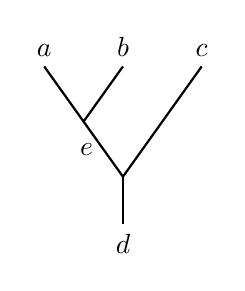
\begin{tikzpicture}[thick, baseline=(current bounding box.center)]
  \draw (0,2) node[above] {$a$} -- (0.5,1.3) -- (1,2) node[above] {$b$};
  \draw (0.5,1.3) -- node[left] {$e$} (1,0.6) -- (2,2) node[above] {$c$};
  \draw (1,0.6) -- (1,0) node[below] {$d$};
\end{tikzpicture}
\;=\; \sum_f \bigl[F^{abc}_d\bigr]_{ef}
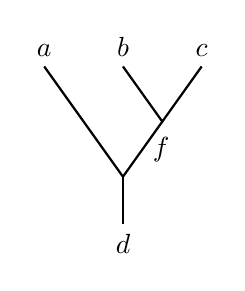
\begin{tikzpicture}[thick, baseline=(current bounding box.center)]
  \draw (0,2) node[above] {$a$} -- (1,0.6);
  \draw (1,2) node[above] {$b$} -- (1.5,1.3) -- (2,2) node[above] {$c$};
  \draw (1.5,1.3) -- node[right] {$f$} (1,0.6);
  \draw (1,0.6) -- (1,0) node[below] {$d$};
\end{tikzpicture}$
